\usetikzlibrary{arrows.meta,positioning,fit,backgrounds,calc,patterns}
\definecolor{ink}{HTML}{1F2933}
\definecolor{train}{HTML}{B45309}
\definecolor{frozen}{HTML}{0369A1}
\definecolor{good}{HTML}{15803D}
\tikzset{mod/.style={draw, rounded corners=2pt, minimum height=8mm, minimum width=20mm, text width=20mm, align=center, font=\small, inner sep=2pt, execute at begin node=\strut, text=ink}, train/.style={mod, fill=train!10, draw=train!75!ink}, frozen/.style={mod, fill=frozen!10, draw=frozen!75!ink}, plain/.style={mod, fill=ink!4, draw=ink!35}, emb/.style={draw=ink!35, fill=ink!4, rounded corners=9pt, minimum height=7mm, minimum width=16mm, align=center, font=\footnotesize, inner sep=3pt, execute at begin node=\strut, text=ink}, lossbox/.style={mod, fill=red!7, draw=red!55!ink, text width=22mm, minimum width=26mm}, objbox/.style={draw=good!70!ink, fill=good!8, rounded corners=3pt, inner sep=6pt, align=center, text=ink}, flow/.style={-{Latex[length=2mm,width=1.4mm]}, thick, draw=ink!75, shorten >=1pt, shorten <=1pt}, grad/.style={-{Latex[length=2mm,width=1.4mm]}, thick, dashed, draw=train!80!ink, shorten >=1pt, shorten <=1pt}, ema/.style={-{Latex[length=2mm,width=1.4mm]}, thick, dashed, draw=frozen!80!ink, shorten >=1pt, shorten <=1pt}, pen/.style={-{Latex[length=1.8mm,width=1.2mm]}, thick, dashed, draw=ink!70, shorten >=1pt, shorten <=1pt}, lbl/.style={font=\scriptsize, text=ink!85, inner sep=1.5pt, fill=white, rounded corners=1pt}, stop/.style={circle, fill=white, draw=ink!70, inner sep=0.4pt, font=\scriptsize, text=ink}}
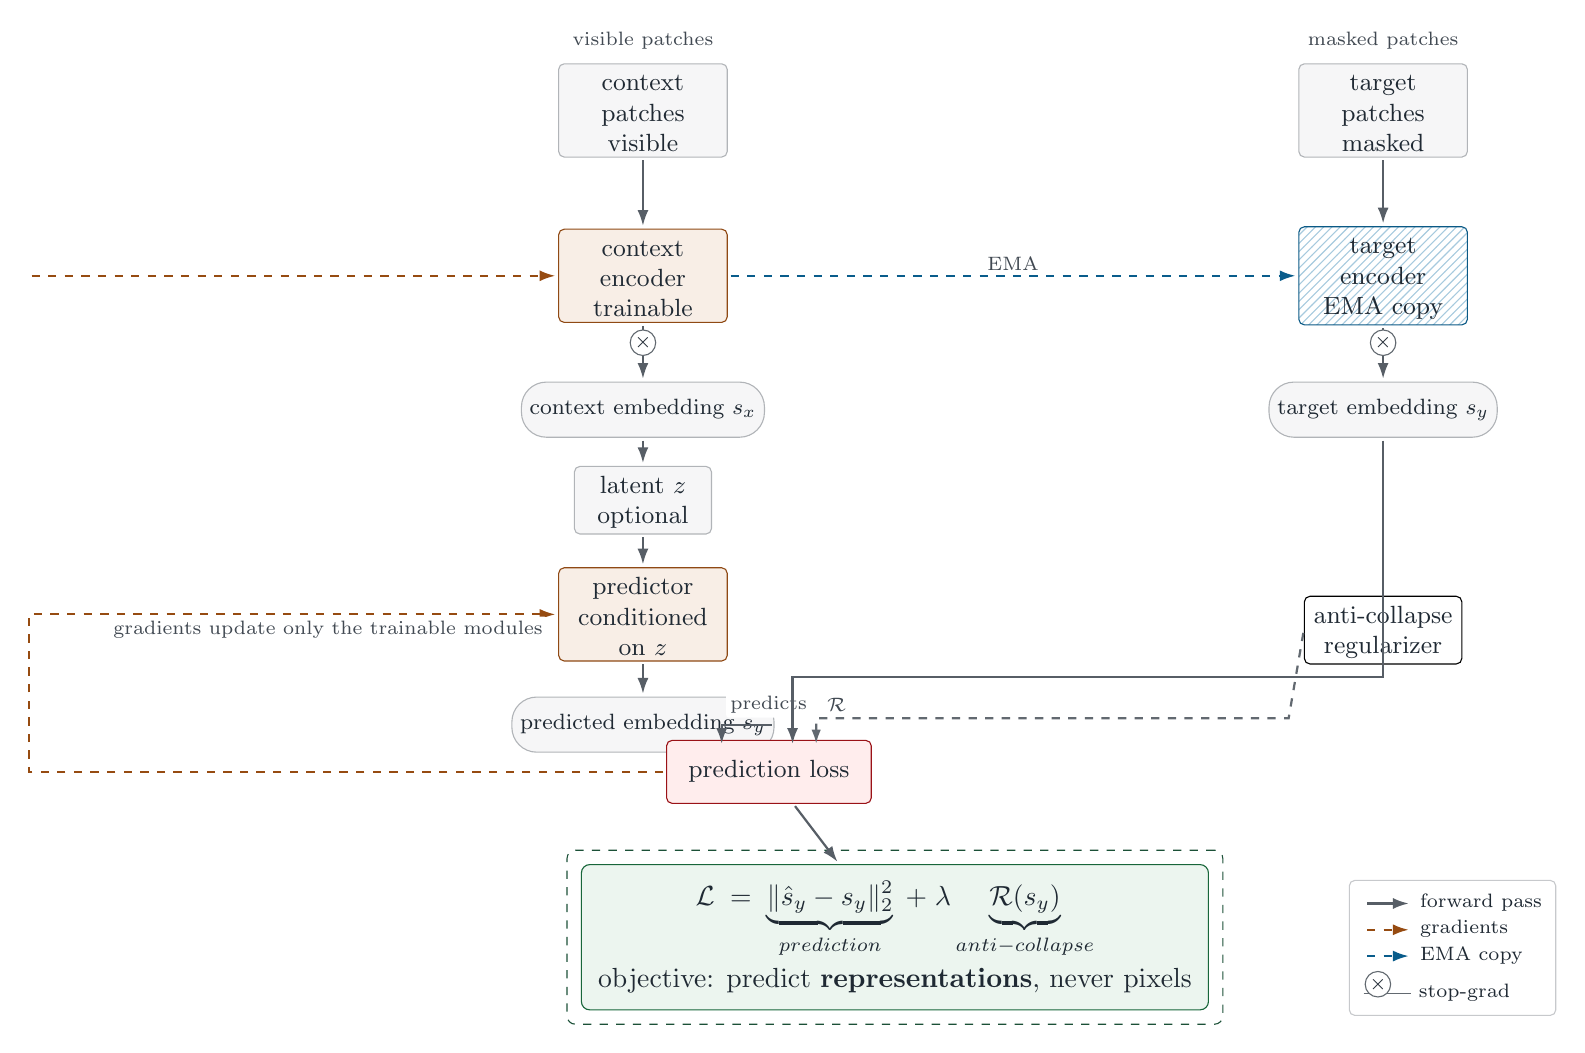
\begin{tikzpicture}[x=1cm, y=1cm]
  \node[plain] (x) at (0,0) {context patches\\ visible};
  \node[plain] (y) at (9.4,0) {target patches\\ masked};
  \node[train] (ex) at (0,-2.1) {context encoder\\ trainable};
  \node[frozen, pattern=north east lines, pattern color=frozen!35] (ey) at (9.4,-2.1) {target encoder\\ EMA copy};
  \node[emb] (sx) at (0,-3.8) {context embedding $s_x$};
  \node[emb] (sy) at (9.4,-3.8) {target embedding $s_y$};
  \node[plain, minimum width=16mm, text width=16mm] (z) at (0,-4.95) {latent $z$\\ optional};
  \node[train] (p) at (0,-6.4) {predictor\\ conditioned on $z$};
  \node[emb] (sh) at (0,-7.8) {predicted embedding $\hat{s}_y$};
  \node[mod, minimum width=20mm, text width=18mm] (reg) at (9.4,-6.6) {anti-collapse\\ regularizer};
  \node[lossbox] (loss) at (1.6,-8.4) {prediction loss};
  \node[objbox] (goal) at (3.2,-10.5) {$\mathcal{L} \;=\; \underbrace{\|\hat{s}_y - s_y\|_2^2}_{\text{prediction}} \;+\; \lambda \underbrace{\mathcal{R}(s_y)}_{\text{anti-collapse}}$\\[3pt] objective: predict \textbf{representations}, never pixels};
  \node[lbl, anchor=south] at (0,0.72) {visible patches};
  \node[lbl, anchor=south] at (9.4,0.72) {masked patches};
  \draw[flow] (x) -- (ex);
  \draw[flow] (y) -- (ey);
  \draw[flow] (ex) -- (sx);
  \draw[flow] (ey) -- (sy);
  \node[stop] at (0,-2.95) {$\times$};
  \node[stop] at (9.4,-2.95) {$\times$};
  \draw[flow] (sx) -- (z);
  \draw[flow] (z) -- (p);
  \draw[flow] (p) -- (sh);
  \draw[flow] (sh.east) -- (1.0,-7.8) -- (1.0,-8.08);
  \node[lbl, anchor=west] at (1.05,-7.55) {predicts};
  \draw[flow] (sy.south) -- (9.4,-7.2) -- (1.9,-7.2) -- (1.9,-8.08);
  \draw[flow] (loss) -- (goal);
  \draw[pen] (reg.west) -- (8.2,-7.72) -- (2.2,-7.72) -- (2.2,-8.08);
  \node[lbl, anchor=west] at (2.28,-7.55) {$\mathcal{R}$};
  \draw[ema] (ex.east) -- node[lbl, above] {EMA} (ey.west);
  \draw[grad] (loss.west) -- (-7.8,-8.4) -- (-7.8,-6.4) -- (p.west);
  \draw[grad] (-7.8,-2.1) -- (ex.west);
  \node[lbl, anchor=north] at (-4.0,-6.42) {gradients update only the trainable modules};
  \begin{pgfonlayer}{background}
    \node[fit=(goal), draw=good!45!ink, dashed, rounded corners=3pt, inner sep=5pt, fill=none] {};
  \end{pgfonlayer}
  \node[draw=ink!25, rounded corners=2pt, inner sep=5pt, align=left, font=\scriptsize, text=ink, fill=white, anchor=south east] at (11.6,-11.5)
    {\tikz[baseline=-0.5ex]{\draw[flow] (0,0)--(6mm,0);}~forward pass\\[1.5pt]
     \tikz[baseline=-0.5ex]{\draw[grad] (0,0)--(6mm,0);}~gradients\\[1.5pt]
     \tikz[baseline=-0.5ex]{\draw[ema] (0,0)--(6mm,0);}~EMA copy\\[1.5pt]
     \tikz[baseline=-0.5ex]{\draw[draw=ink!70] (0,0)--(6mm,0); \node[stop, inner sep=0.4pt] at (3mm,0) {$\times$};}~stop-grad};
\end{tikzpicture}